\documentclass{article}
\usepackage[utf8]{inputenc} 
\usepackage[spanish]{babel}
\usepackage{url} 
\usepackage{enumerate}
\usepackage{graphicx}
\usepackage{float}
\usepackage{multicol}
\usepackage[absolute,overlay]{textpos}
  \setlength{\TPHorizModule}{1mm}
  \setlength{\TPVertModule}{1mm}
\usepackage{colortbl}
\usepackage[colorlinks=true,linkcolor=black,urlcolor=black, citecolor=black]{hyperref}
\usepackage[top=30mm,bottom=30mm,inner=30mm,outer=20mm,asymmetric]{geometry}
\newcommand{\degree}{\ensuremath{^\circ}}
\begin{document}
\section*{Gráficas de resultados de la ejecución de los algoritmos con las vistas minables construidas.}
En este documento se presentan los resultados de ejecutar las vistas minables creadas en la sección 4.2 del trabajo de grado Aplicación para la predicción de resultados en la prueba Saber 11\degree.\\

Se presentan los valores de precisión y exhaustividad (Recall) que se obtuvo al ejecutar cada algoritmo con una cantidad de 1000  instancias contenidas en los archivos de evaluación. En el área derecha de cada gráfica se indica el significado de cada punto en la gráfica. Cada punto representa un algoritmo y la cantidad de instancias con las que se entrenó ese algoritmo. Por ejemplo, en la figura \ref{fig:figura1} se observa J48 – 1000, lo cual quiere decir que indica la precisión y la exhaustividad que obtuvo el algoritmo J48 entrenado con 1000 instancias.\\

Para el caso de los k vecinos más cercanos (IBK), se presentan los resultados tanto para la ejecución con k=1 como para la ejecución con k=2.\\

Los nombres de los algoritmos presentados en las gráficas, son los nombres de las librerías que los ejecutan en Weka. C4.5 es J48, k vecinos más cercanos es IBK, Naive Bayes es Naive y la red neural de funciones de base radial es RBF.\\
\begin{textblock}{80}(25,120)
\begin{figure}[!htb]
\begin{centering}
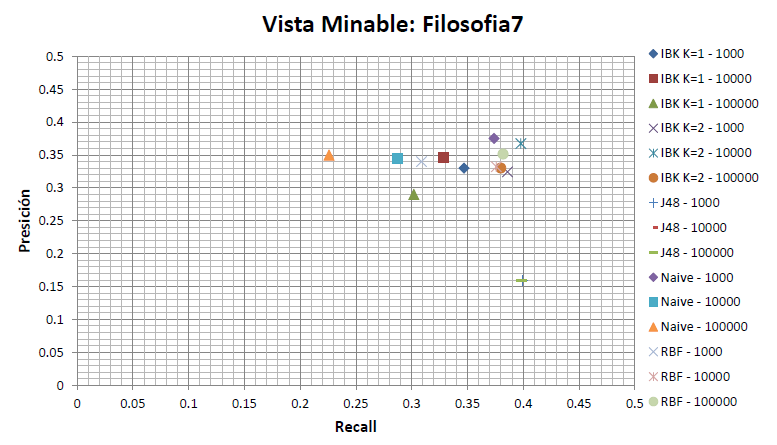
\includegraphics[scale=0.4]{filosofia7}
\par\end{centering}
\caption{Precision y recall obtenidos al evaluar los clasificadores entrenados usando la vista minable Filosofia7.}
\label{fig:figura1}
\end{figure}
\end{textblock}

\begin{textblock}{80}(110,120)
\begin{figure}[!htb]
\begin{centering}
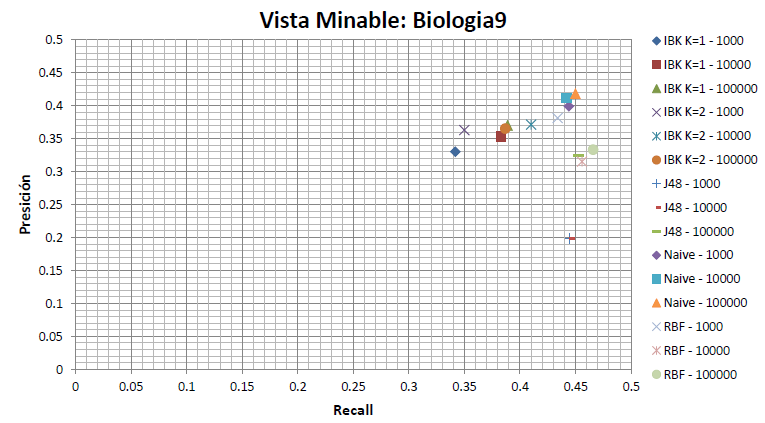
\includegraphics[scale=0.4]{biologia9}
\par\end{centering}
\caption{Precision y recall obtenidos al evaluar los clasificadores entrenados usando la vista minable Biologia9.}
\label{fig:figura2}
\end{figure}
\end{textblock}

\begin{textblock}{80}(25,186)
\begin{figure}[!htb]
\begin{centering}
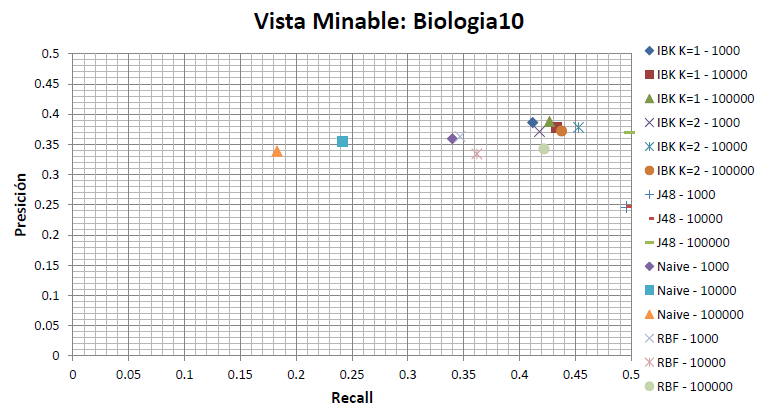
\includegraphics[scale=0.4]{biologia10}
\par\end{centering}
\caption{Precision y recall obtenidos al evaluar los clasificadores entrenados usando la vista minable Biologia10.}
\label{fig:figura3}
\end{figure}
\end{textblock}

\begin{textblock}{80}(110,185)
\begin{figure}[!htb]
\begin{centering}
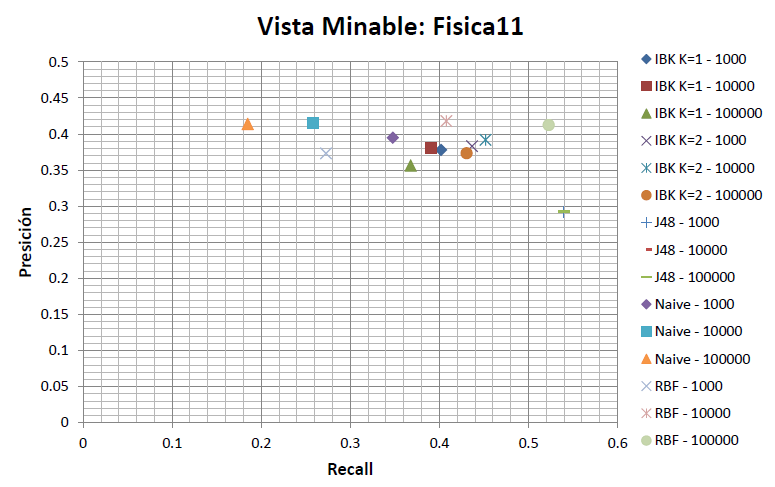
\includegraphics[scale=0.4]{fisica11}
\par\end{centering}
\caption{Precision y recall obtenidos al evaluar los clasificadores entrenados usando la vista minable Fisica11.}
\label{fig:figura4}
\end{figure}
\end{textblock}

\clearpage

\begin{textblock}{80}(25,30)
\begin{figure}[!htb]
\begin{centering}
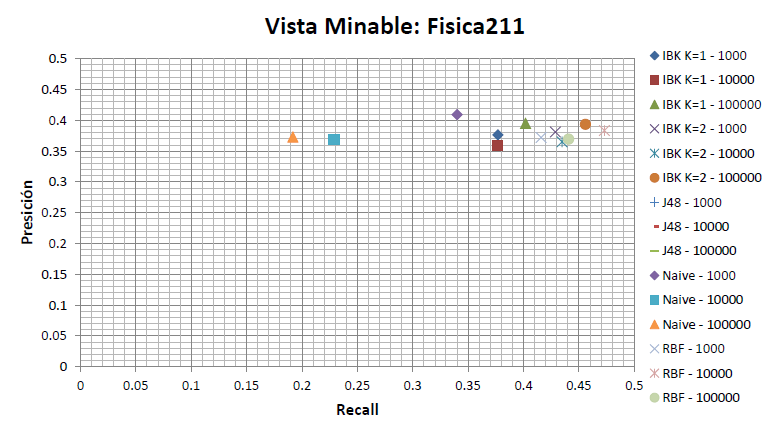
\includegraphics[scale=0.4]{fisica211}
\par\end{centering}
\caption{Precision y recall obtenidos al evaluar los clasificadores entrenados usando la vista minable Fisica211.}
\label{fig:figura5}
\end{figure}
\end{textblock}

\begin{textblock}{80}(110,30)
\begin{figure}[!htb]
\begin{centering}
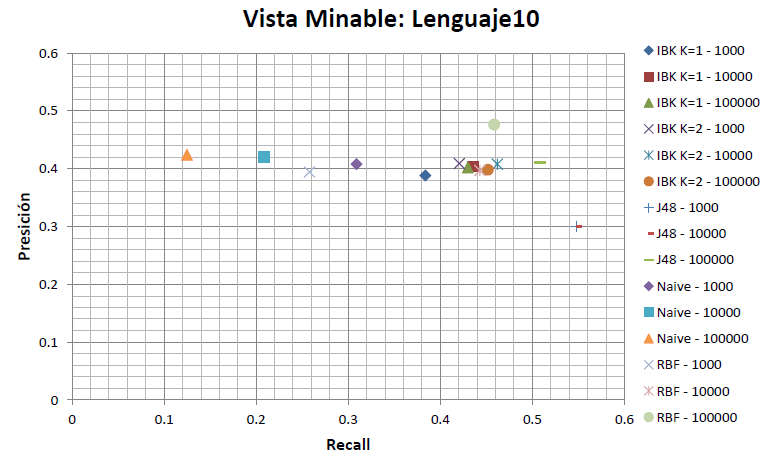
\includegraphics[scale=0.4]{lenguaje10}
\par\end{centering}
\caption{Precision y recall obtenidos al evaluar los clasificadores entrenados usando la vista minable Lenguaje10.}
\label{fig:figura6}
\end{figure}
\end{textblock}

\begin{textblock}{80}(25,100)
\begin{figure}[!htb]
\begin{centering}
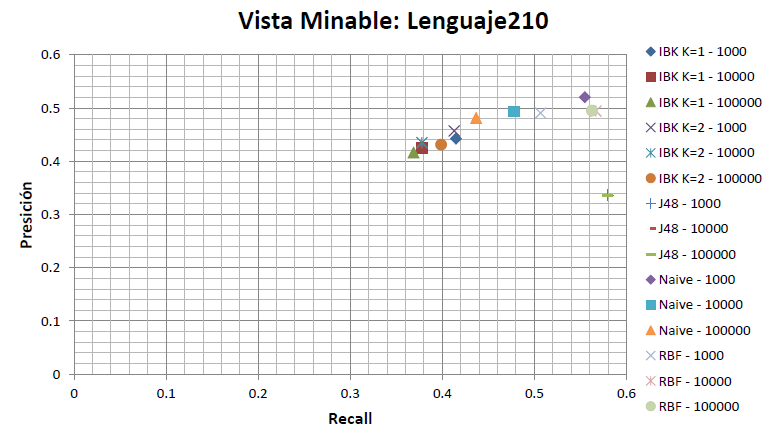
\includegraphics[scale=0.4]{lenguaje210}
\par\end{centering}
\caption{Precision y recall obtenidos al evaluar los clasificadores entrenados usando la vista minable Lenguaje210.}
\label{fig:figura7}
\end{figure}
\end{textblock}

\begin{textblock}{80}(110,100)
\begin{figure}[!htb]
\begin{centering}
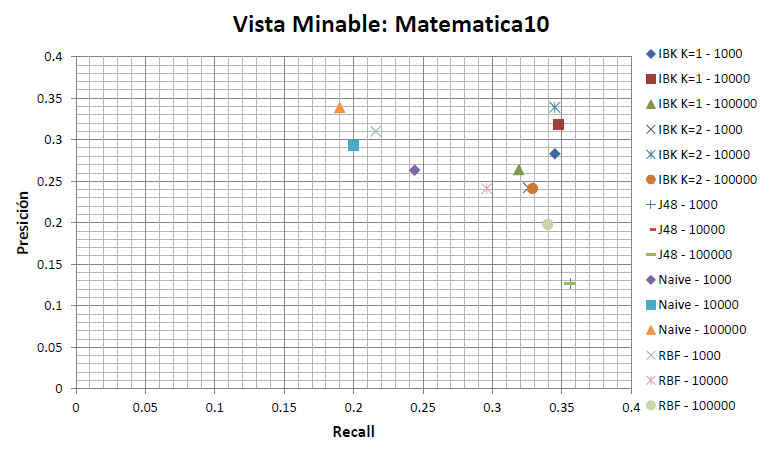
\includegraphics[scale=0.4]{matematica10}
\par\end{centering}
\caption{Precision y recall obtenidos al evaluar los clasificadores entrenados usando la vista minable Matematica10.}
\label{fig:figura8}
\end{figure}
\end{textblock}

\begin{textblock}{80}(25,170)
\begin{figure}[!htb]
\begin{centering}
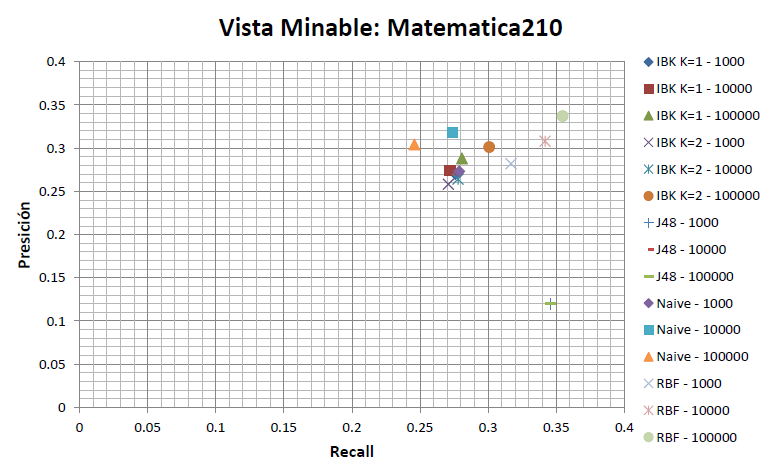
\includegraphics[scale=0.4]{matematica210}
\par\end{centering}
\caption{Precision y recall obtenidos al evaluar los clasificadores entrenados usando la vista minable Matematica210.}
\label{fig:figura9}
\end{figure}
\end{textblock}

\begin{textblock}{80}(110,170)
\begin{figure}[!htb]
\begin{centering}
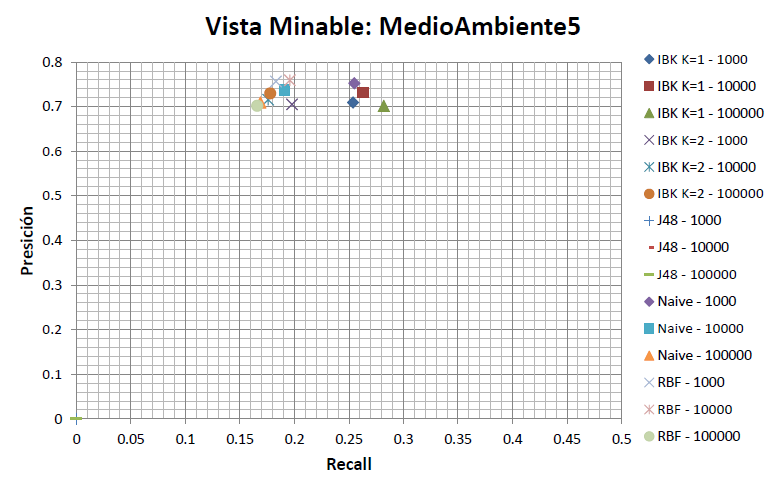
\includegraphics[scale=0.4]{medioambiente5}
\par\end{centering}
\caption{Precision y recall obtenidos al evaluar los clasificadores entrenados usando la vista minable MedioAmbiente5.}
\label{fig:figura10}
\end{figure}
\end{textblock}
\null
\clearpage

\begin{textblock}{80}(25,30)
\begin{figure}[!htb]
\begin{centering}
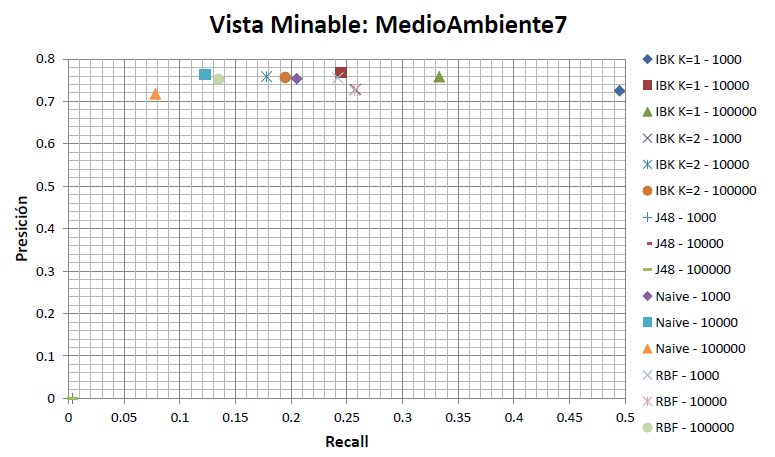
\includegraphics[scale=0.4]{medioambiente7}
\par\end{centering}
\caption{Precision y recall obtenidos al evaluar los clasificadores entrenados usando la vista minable MedioAmbiente7.}
\label{fig:figura11}
\end{figure}
\end{textblock}

\begin{textblock}{80}(110,30)
\begin{figure}[!htb]
\begin{centering}
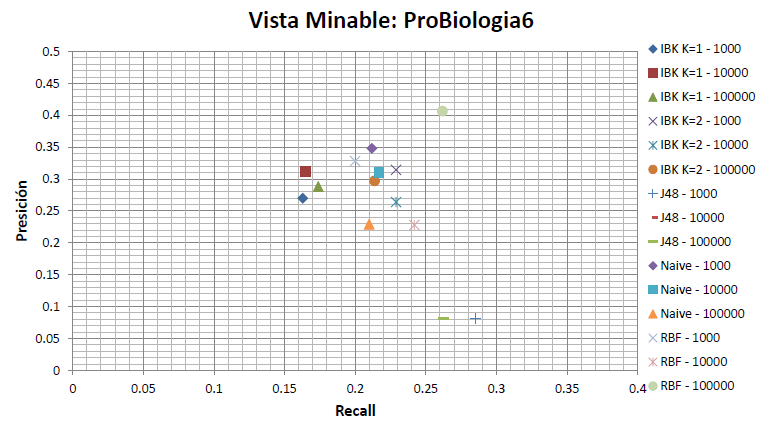
\includegraphics[scale=0.4]{probiologia6}
\par\end{centering}
\caption{Precision y recall obtenidos al evaluar los clasificadores entrenados usando la vista minable ProBiologia6.}
\label{fig:figura12}
\end{figure}
\end{textblock}

\begin{textblock}{80}(25,100)
\begin{figure}[!htb]
\begin{centering}
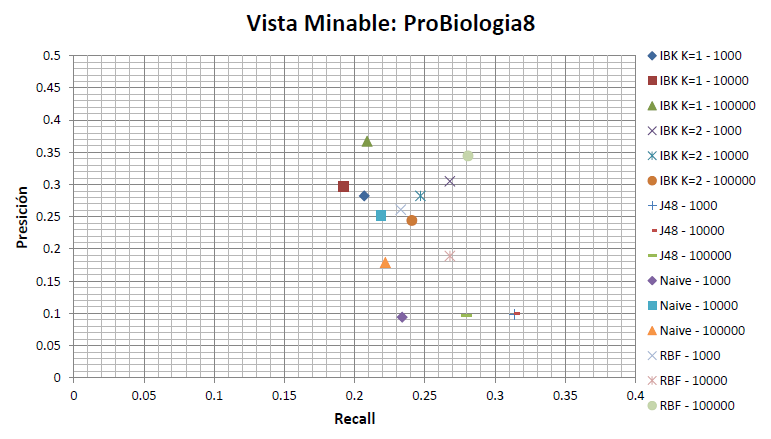
\includegraphics[scale=0.4]{probiologia8}
\par\end{centering}
\caption{Precision y recall obtenidos al evaluar los clasificadores entrenados usando la vista minable ProBiologia8.}
\label{fig:figura13}
\end{figure}
\end{textblock}

\begin{textblock}{80}(110,100)
\begin{figure}[!htb]
\begin{centering}
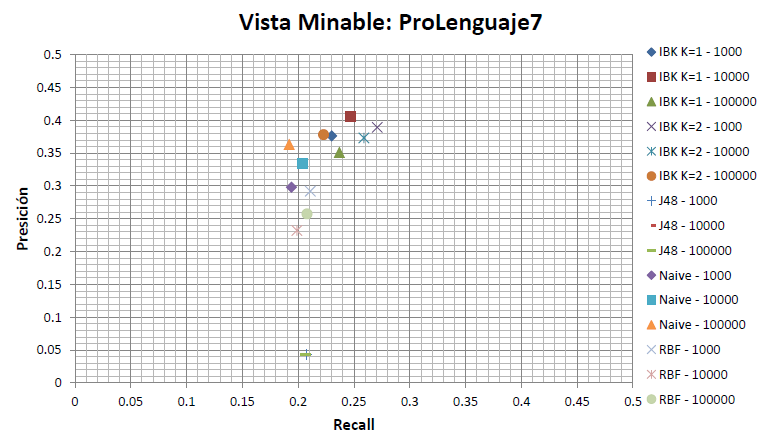
\includegraphics[scale=0.4]{prolenguaje7}
\par\end{centering}
\caption{Precision y recall obtenidos al evaluar los clasificadores entrenados usando la vista minable ProLenguaje7.}
\label{fig:figura14}
\end{figure}
\end{textblock}

\begin{textblock}{80}(25,170)
\begin{figure}[!htb]
\begin{centering}
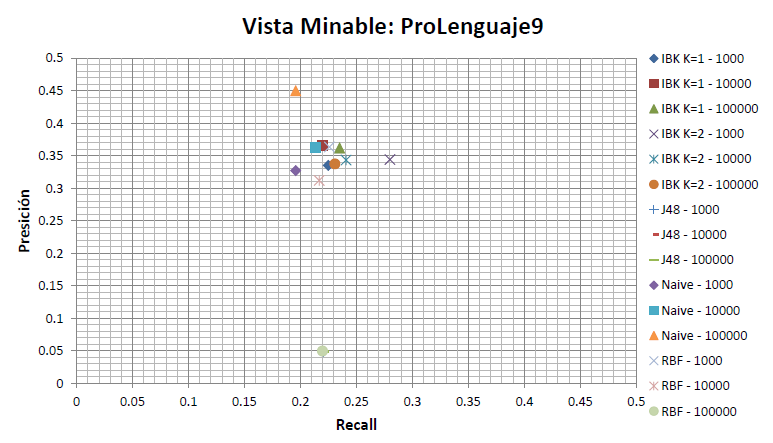
\includegraphics[scale=0.4]{prolenguaje9}
\par\end{centering}
\caption{Precision y recall obtenidos al evaluar los clasificadores entrenados usando la vista minable ProLenguaje9.}
\label{fig:figura15}
\end{figure}
\end{textblock}

\begin{textblock}{80}(110,170)
\begin{figure}[!htb]
\begin{centering}
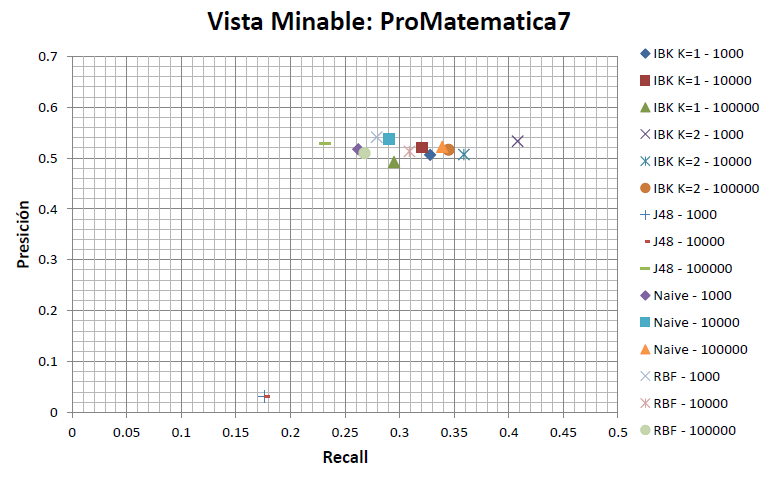
\includegraphics[scale=0.4]{promatematica7}
\par\end{centering}
\caption{Precision y recall obtenidos al evaluar los clasificadores entrenados usando la vista minable ProMatematica7.}
\label{fig:figura16}
\end{figure}
\end{textblock}
\null
\newpage
\begin{textblock}{80}(25,30)
\begin{figure}[!htb]
\begin{centering}
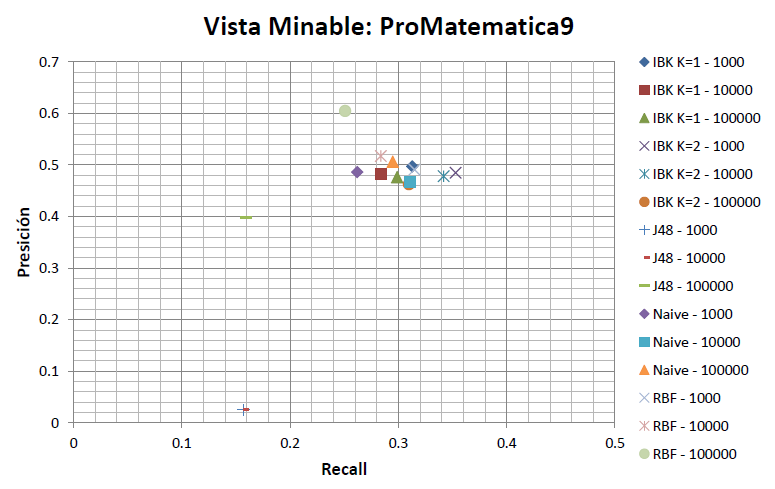
\includegraphics[scale=0.4]{promatematica9}
\par\end{centering}
\caption{Precision y recall obtenidos al evaluar los clasificadores entrenados usando la vista minable ProMatematica9.}
\label{fig:figura17}
\end{figure}
\end{textblock}

\begin{textblock}{80}(110,30)
\begin{figure}[!htb]
\begin{centering}
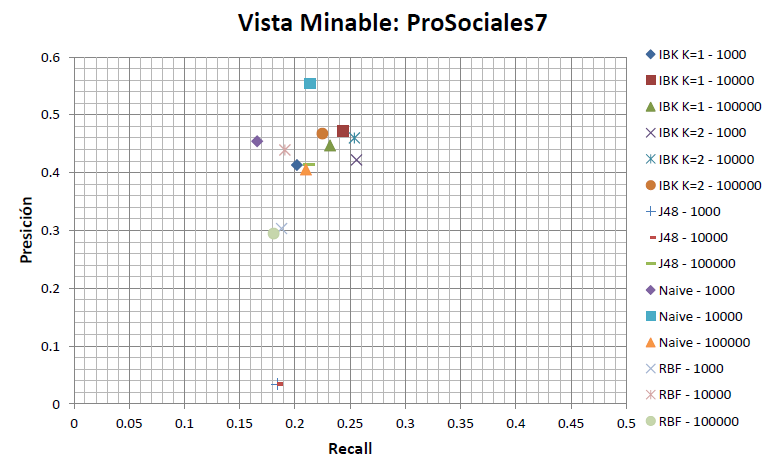
\includegraphics[scale=0.4]{prosociales7}
\par\end{centering}
\caption{Precision y recall obtenidos al evaluar los clasificadores entrenados usando la vista minable ProSociales7.}
\label{fig:figura18}
\end{figure}
\end{textblock}

\begin{textblock}{80}(25,105)
\begin{figure}[!htb]
\begin{centering}
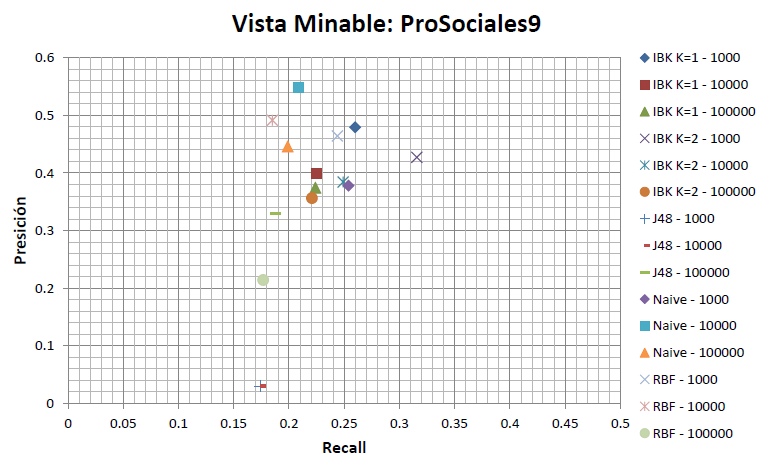
\includegraphics[scale=0.4]{prosociales9}
\par\end{centering}
\caption{Precision y recall obtenidos al evaluar los clasificadores entrenados usando la vista minable ProSociales9.}
\label{fig:figura19}
\end{figure}
\end{textblock}

\begin{textblock}{80}(110,105)
\begin{figure}[!htb]
\begin{centering}
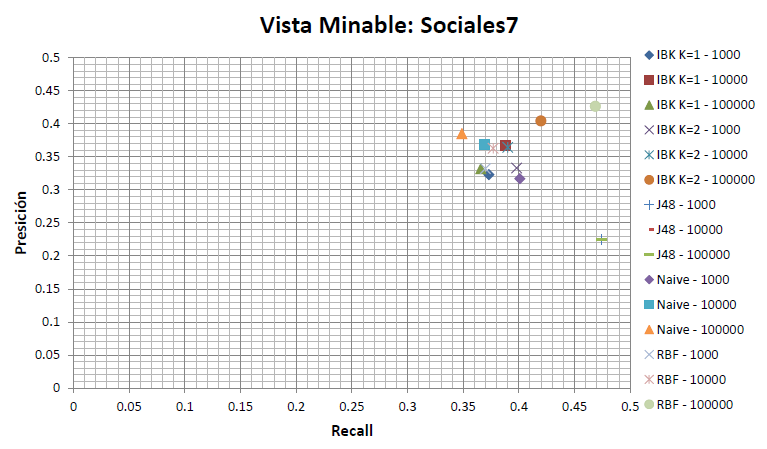
\includegraphics[scale=0.4]{sociales7}
\par\end{centering}
\caption{Precision y recall obtenidos al evaluar los clasificadores entrenados usando la vista minable Sociales7.}
\label{fig:figura20}
\end{figure}
\end{textblock}

\begin{textblock}{80}(25,180)
\begin{figure}[!htb]
\begin{centering}
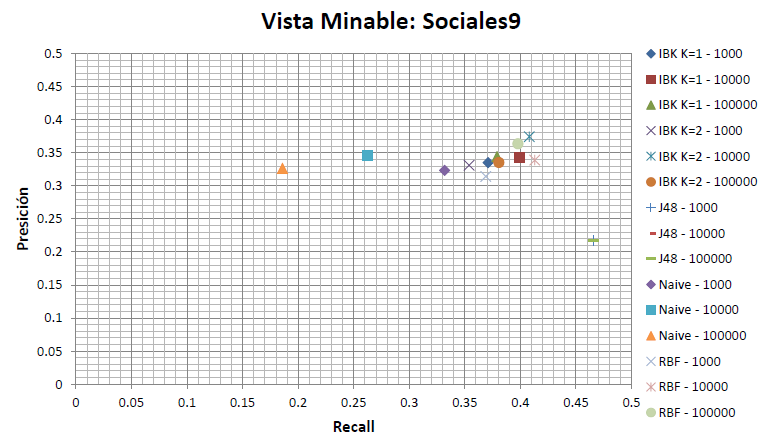
\includegraphics[scale=0.4]{sociales9}
\par\end{centering}
\caption{Precision y recall obtenidos al evaluar los clasificadores entrenados usando la vista minable Sociales9.}
\label{fig:figura21}
\end{figure}
\end{textblock}

\begin{textblock}{80}(110,180)
\begin{figure}[!htb]
\begin{centering}
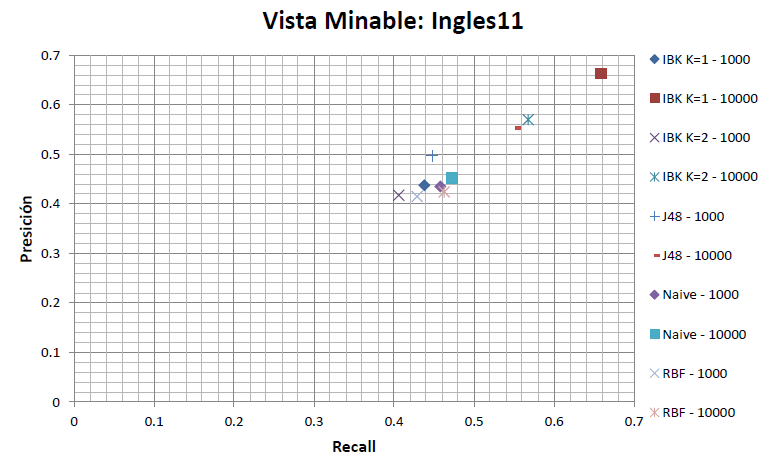
\includegraphics[scale=0.4]{ingles11}
\par\end{centering}
\caption{Precision y recall obtenidos al evaluar los clasificadores entrenados usando la vista minable Ingles11.}
\label{fig:figura22}
\end{figure}
\end{textblock}
\null
\newpage
\begin{textblock}{80}(25,30)
\begin{figure}[!htb]
\begin{centering}
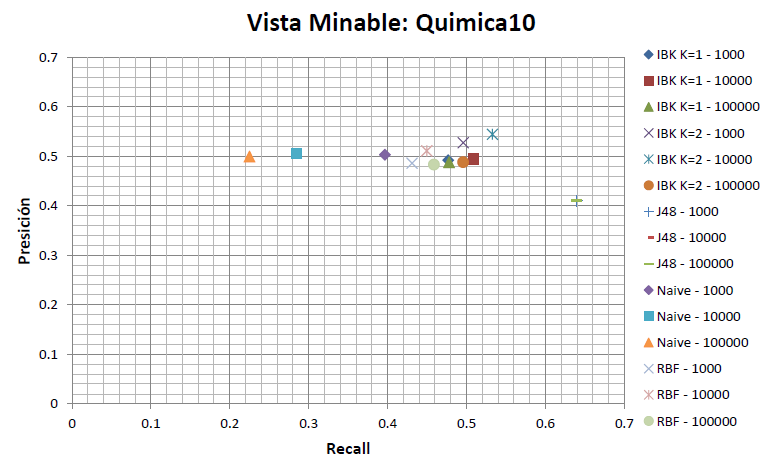
\includegraphics[scale=0.4]{quimica10}
\par\end{centering}
\caption{Precision y recall obtenidos al evaluar los clasificadores entrenados usando la vista minable Quimica10.}
\label{fig:figura23}
\end{figure}
\end{textblock}

\begin{textblock}{80}(110,30)
\begin{figure}[!htb]
\begin{centering}
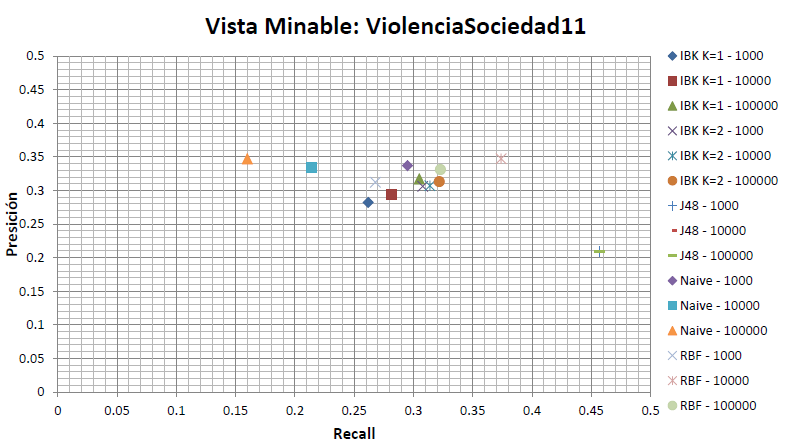
\includegraphics[scale=0.4]{violenciasociedad11}
\par\end{centering}
\caption{Precision y recall obtenidos al evaluar los clasificadores entrenados usando la vista minable ViolenciaSociedad11.}
\label{fig:figura24}
\end{figure}
\end{textblock}
\end{document}